\documentclass[12pt, oneside]{article}   	% use "amsart" instead of "article" for AMSLaTeX format

%%%%%%%%%%%%%%%%%%%%%%%%%%%%%%%%%%%%%%%%%%%%%%%%%%%%
% set up packages, geometry
%%%%%%%%%%%%%%%%%%%%%%%%%%%%%%%%%%%%%%%%%%%%%%%%%%%%
\usepackage{geometry, textcomp, amsmath, graphicx, amssymb,fancyhdr,subcaption,bm}                
	
\geometry{letterpaper, marginparwidth=60pt}                   		
\usepackage[superscript,noadjust]{cite} % puts dash in citations to abbreviate
%\usepackage [autostyle, english = american]{csquotes} % sets US-style quotes
%\MakeOuterQuote{"} % sets quote style
          
\usepackage{lineno}
\usepackage{pdfpages}
\usepackage{etoolbox}
\usepackage{float,color}
\usepackage{soul}

\begin{document}

\section*{Figures}
\subsection*{Belowground}

%%%%%%%%%%%%%%%%%%%%%%%%%%%%%%%%%%%%%%%%%%%%%%%%%%%%
% Conceptual figures
%%%%%%%%%%%%%%%%%%%%%%%%%%%%%%%%%%%%%%%%%%%%%%%%%%%%

 \begin{figure}[!h]
   \centering
       %\includegraphics[page=1,width=1\textwidth]{../../manuscript/figures/seed-bag-figure.pdf}  
       \includegraphics[page=1,width=1\textwidth]{seed-bag-figure.pdf}  
    \caption{ Summary of the seed bag burial experiments and viability trials. \hl{Figure will be labeled as (A: seed bag trials , B: viability trials, C: germination probability, D: survival probability. }. (A) The gray panel contains a graphical representation of the seed bag trials. Seeds were buried at the start of each experiment (100 seeds in month 0). Seed bags were unearthed and intact seeds ($y_{\cdot \cdot}$) and germinants ($y_{\mathrm{g},\cdot}$ counted. The graph below the panel shows a hypothetical survival function associated with persistence of seeds in the soil seed bank. (B) The gray panel contains a graphical representation of the viability trials. Seeds were tested in two rounds; germination trials were performed and then some or all of the ungerminated seeds were tested for viability. The graph below the panel shows hypothetical data from a series of viability trials and the interpolated, inferred viabilities at times when viability was unobserved. (C) Age-specific germination probably is summarized in three ways. (D) The graph shows the survival function for persistence of seeds in the soil seed bank (black line) and the estimated discrete survival probabilities for persistence and viability of seeds (orange points). }
 \label{fig:seed-bag-experiments}
\end{figure}

\clearpage
\newpage

%%%%%%%%%%%%%%%%%%%%%%%%%%%%%%%%%%%%%%%%%%%%%%%%%%%%
%%%%%%%%%%%%%%%%%%%%%%%%%%%%%%%%%%%%%%%%%%%%%%%%%%%%
% Parameter estimation
%%%%%%%%%%%%%%%%%%%%%%%%%%%%%%%%%%%%%%%%%%%%%%%%%%%%
%%%%%%%%%%%%%%%%%%%%%%%%%%%%%%%%%%%%%%%%%%%%%%%%%%%%


%%%%%%%%%%%%%%%%%%%%%%%%%%%%%%%%%%%%%%%%%%%%%%%%%%%%
% Survival function: continuous component
%%%%%%%%%%%%%%%%%%%%%%%%%%%%%%%%%%%%%%%%%%%%%%%%%%%%

 \begin{figure}[!h]
   \centering
       \includegraphics[page=2,width=1\textwidth]{../../figures/survival-function-population.pdf}  
    \caption{ The continuous component of the population-level survival function, summarized for each population by the median and 95\% credible intervals. Credible intervals were constructed by obtaining the posterior probability of survival at each time according to a Weibull survival function, and then calculating the quantiles at each time point.  }
 \label{fig:viability-estimates-population}
\end{figure}

 \begin{figure}[!h]
   \centering
       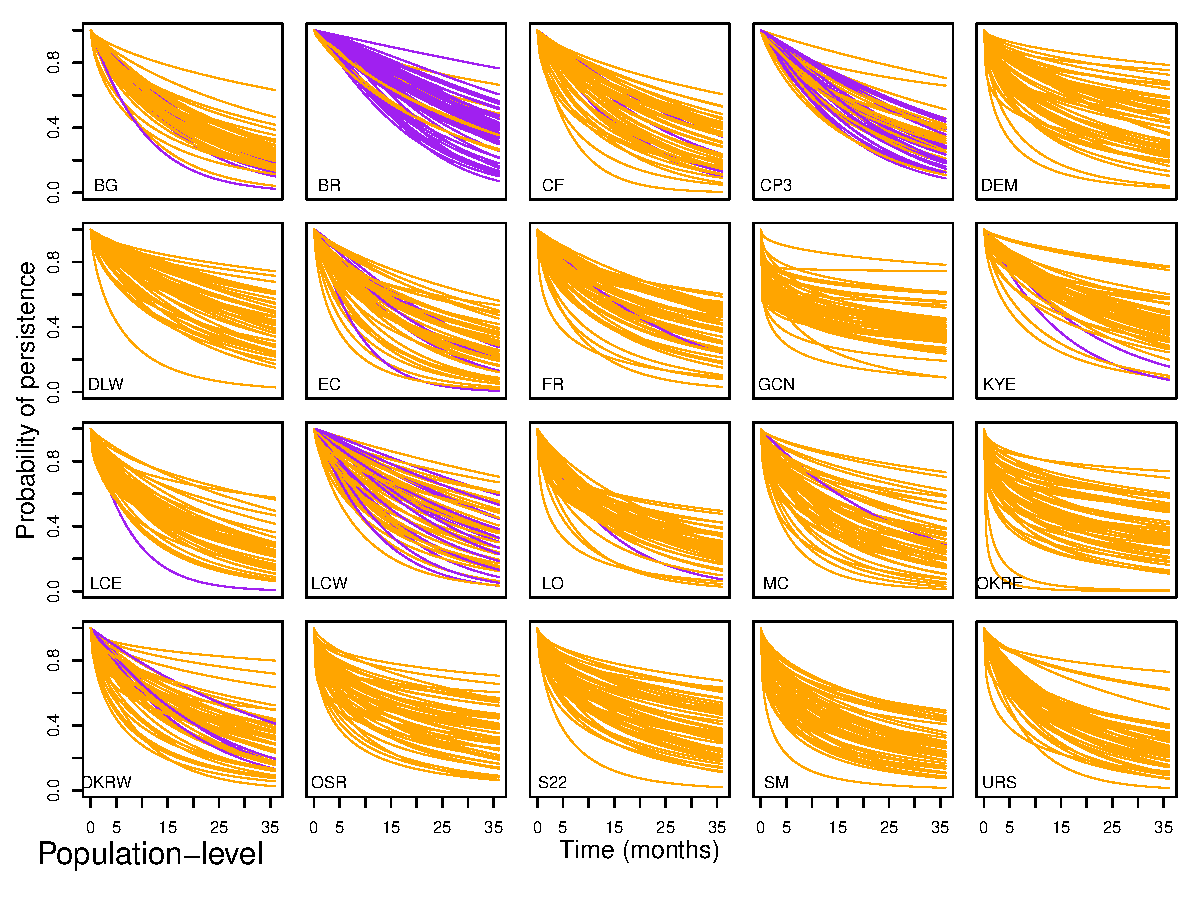
\includegraphics[page=1,width=1\textwidth]{../../figures/survival-function-population.pdf}  
    \caption{ Fifty draws from the continuous component of the population-level survival function. Each line uses one draw from the posteriors for the shape and inverse scale parameters to calculate the probability of survival  over time according to a Weibull survival function. Lines are colored so that samples for which the shape parameter is greater than one are purple, and samples for which the shape parameter is less than one are in orange.    }
 \label{fig:viability-estimates-population}
\end{figure}

 \begin{figure}[!h]
   \centering
       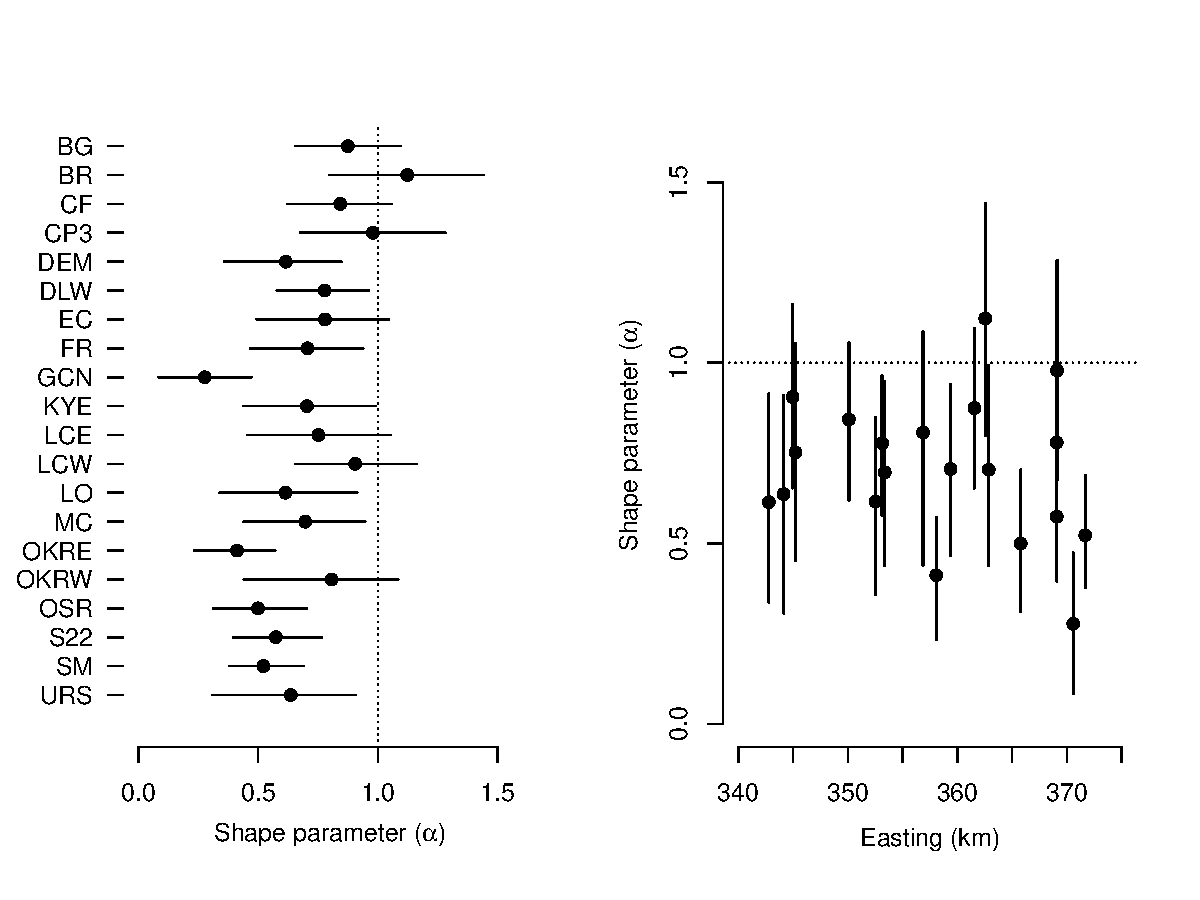
\includegraphics[page=1,width=1\textwidth]{../../figures/survival-function-parms-population.pdf}  
    \caption{ Population-level estimates for the shape parameter ($\alpha$) of the Weibull survival function. }
 \label{fig:viability-estimates-population}
\end{figure}

%%%%%%%%%%%%%%%%%%%%%%%%%%%%%%%%%%%%%%%%%%%%%%%%%%%%
% Survival function: discrete component
%%%%%%%%%%%%%%%%%%%%%%%%%%%%%%%%%%%%%%%%%%%%%%%%%%%%

 \begin{figure}[!h]
   \centering
       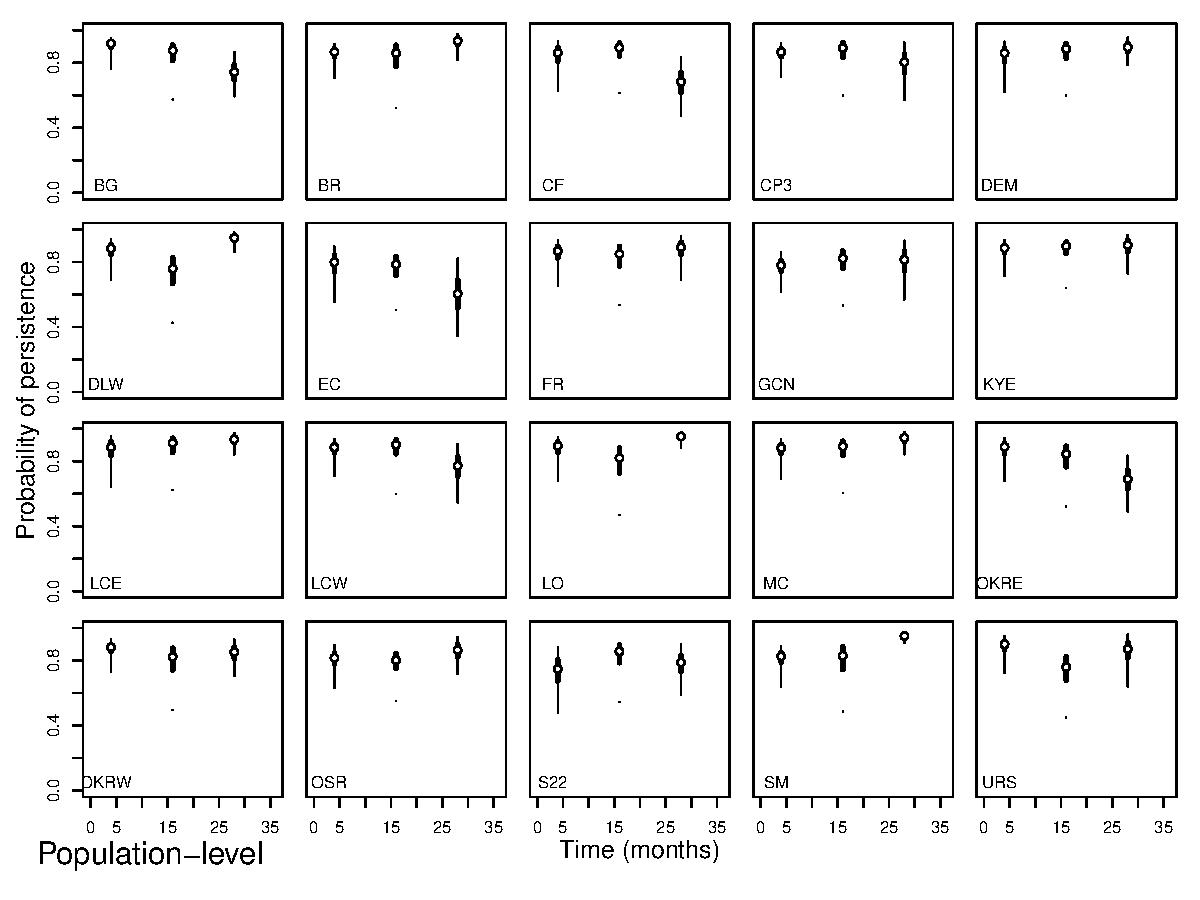
\includegraphics[page=1,width=1\textwidth]{../../figures/survival-function-discrete.pdf}  
    \caption{ The discrete component of the population-level survival function, summarized for each population by the median and 95\% credible intervals. Credible intervals were constructed by obtaining the posterior probability of persistence at each time. Times correspond to the periods at which seeds germinated; the probabilities here are the probabilities that seeds did not germinate.  }
 \label{fig:viability-estimates-population}
\end{figure}

%%%%%%%%%%%%%%%%%%%%%%%%%%%%%%%%%%%%%%%%%%%%%%%%%%%%
% Survival function: compound component and summary
%%%%%%%%%%%%%%%%%%%%%%%%%%%%%%%%%%%%%%%%%%%%%%%%%%%%

 \begin{figure}[!h]
   \centering
       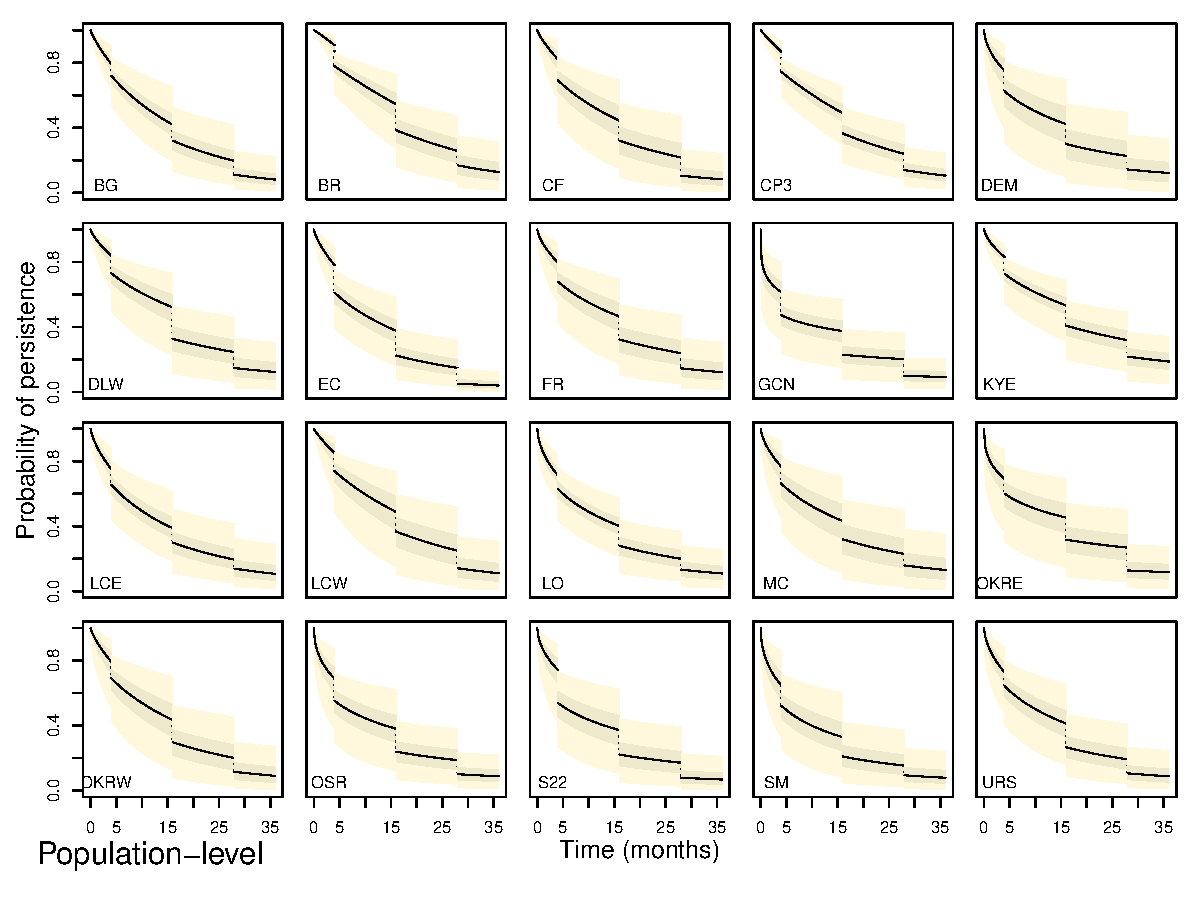
\includegraphics[page=1,width=1\textwidth]{../../figures/survival-function-compound.pdf}  
    \caption{ The combination of the continuous and discrete population-level survival function, summarized for each population by the median and 50\% \& 95\% credible intervals. Credible intervals were constructed by obtaining the posterior probability of persistence at each time. }
 \label{fig:viability-estimates-population}
\end{figure}

%%%%%%%%%%%%%%%%%%%%%%%%%%%%%%%%%%%%%%%%%%%%%%%%%%%%
% Viability
%%%%%%%%%%%%%%%%%%%%%%%%%%%%%%%%%%%%%%%%%%%%%%%%%%%%
 \begin{figure}[!h]
   \centering
       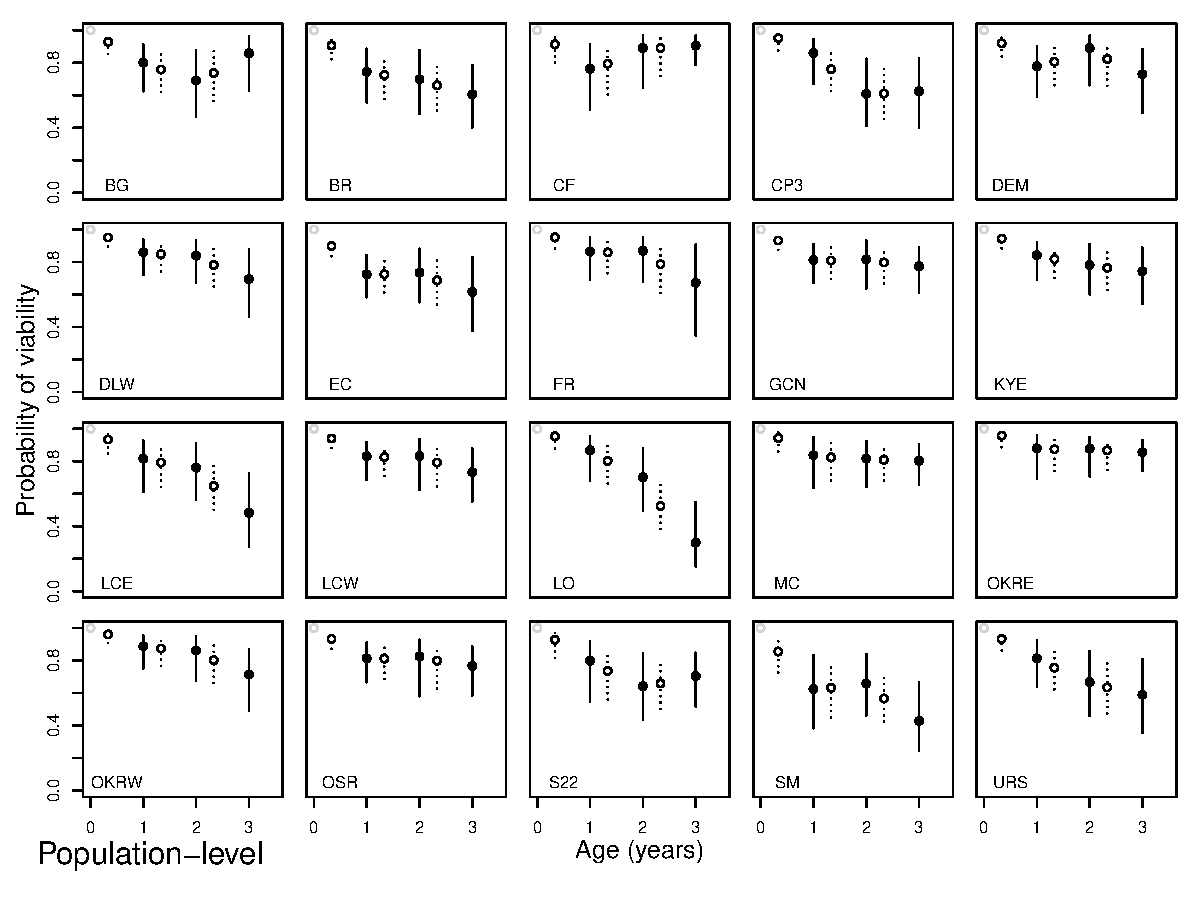
\includegraphics[page=1,width=1\textwidth]{../../figures/viability-estimates-population.pdf}  
    \caption{ Population-level estimates of viability from the 20 study populations. Filled points correspond to viability estimates from October and open points correspond to inferred viability estimates in January, interpolating between estimates as described in the main text. Points are the median of the posterior of viability; lines are the 95\% credible intervals. Three years of data contribute to estimates of viability for 1 year old seeds; two years of data contribute to estimates of viability for 2 year old seeds; one year of data contributes to estimates of viability for 3 year old seeds. }
 \label{fig:viability-estimates-population}
\end{figure}

 \begin{figure}[!h]
   \centering
       \includegraphics[page=2,width=1\textwidth]{../../figures/viability-estimates-population.pdf}  
    \caption{ Population-level estimates of median viability from the 20 study populations over three years. All populations are combined here to facilitate a visual comparison of how estimates of viability change over time across populations. Filled points correspond to viability estimates from October and open points correspond to inferred viability estimates in January, interpolating between estimates as described in the main text. Points are the median of the posterior of viability. Three years of data contribute to estimates of viability for 1 year old seeds; two years of data contribute to estimates of viability for 2 year old seeds; one year of data contributes to estimates of viability for 3 year old seeds.  }
 \label{fig:viability-estimates-population}
\end{figure}

%%%%%%%%%%%%%%%%%%%%%%%%%%%%%%%%%%%%%%%%%%%%%%%%%%%%
% Survival function: incorporating viability
%%%%%%%%%%%%%%%%%%%%%%%%%%%%%%%%%%%%%%%%%%%%%%%%%%%%

 \begin{figure}[!h]
   \centering
       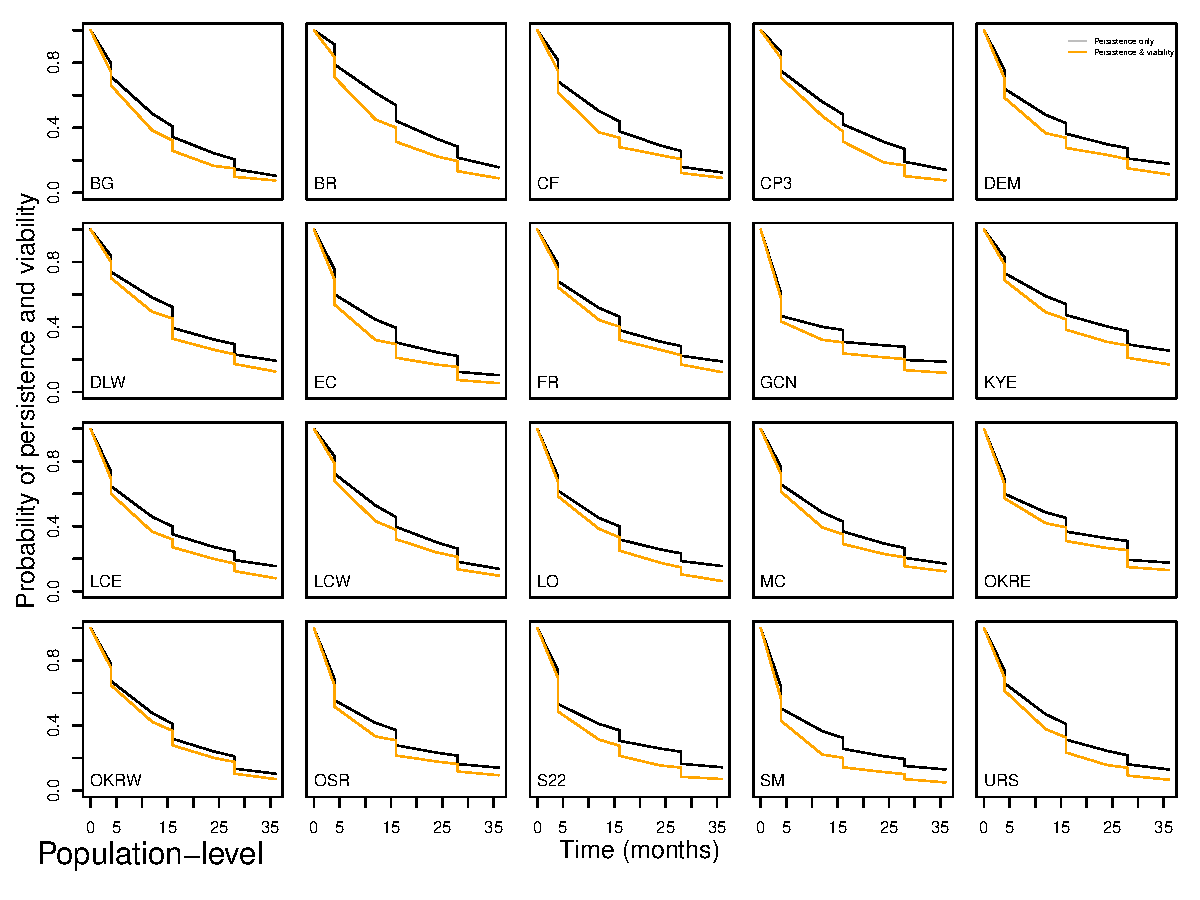
\includegraphics[page=1,width=1\textwidth]{../../figures/survival-function-persistence-viability.pdf}  
    \caption{ Patterns from the discretized survival function with (orange) and without (black) incorporating estimates of viability. The line summarizes the pattern of survival by the median. \hl{To incorporate viability, we discretized estimates of persistence to correspond to times where we observed germination or unearthed the seed bags to perform viability trials in the lab. The survival function is thus no longer continuous; here, we show lines connecting points to illustrate the general patterns of survival.} }
 \label{fig:viability-estimates-population}
\end{figure}

 \begin{figure}[!h]
   \centering
       \includegraphics[page=3,width=1\textwidth]{../../figures/survival-function-persistence-viability.pdf}  
    \caption{ The discretized, population-level survival function for persistence (black) and for persistence and viability (orange), summarized for each population by the median and 95\% credible intervals.  Credible intervals were constructed by obtaining the posterior probability of survival at each time (after an event) from the survival functions for persistence, or for persistence and viability. We discretized the continuous survival function to correspond to times at which we observed germination or unearthed the seed bags to perform viability trials in the lab. The plots show two possible events: (1) loss of seeds from the soil seed bank due to physical destruction or loss of viability and (2) loss of seeds from the soil seed bank due to germination. The first event is represented by solid lines; the second event is represented by dotted lines. }
 \label{fig:viability-estimates-population}
\end{figure}

%%%%%%%%%%%%%%%%%%%%%%%%%%%%%%%%%%%%%%%%%%%%%%%%%%%%
%%%%%%%%%%%%%%%%%%%%%%%%%%%%%%%%%%%%%%%%%%%%%%%%%%%%
% Structured model parameters
%%%%%%%%%%%%%%%%%%%%%%%%%%%%%%%%%%%%%%%%%%%%%%%%%%%%
%%%%%%%%%%%%%%%%%%%%%%%%%%%%%%%%%%%%%%%%%%%%%%%%%%%%

%%%%%%%%%%%%%%%%%%%%%%%%%%%%%%%%%%%%%%%%%%%%%%%%%%%%
% Germination
%%%%%%%%%%%%%%%%%%%%%%%%%%%%%%%%%%%%%%%%%%%%%%%%%%%%

 \begin{figure}[!h]
        \centering
        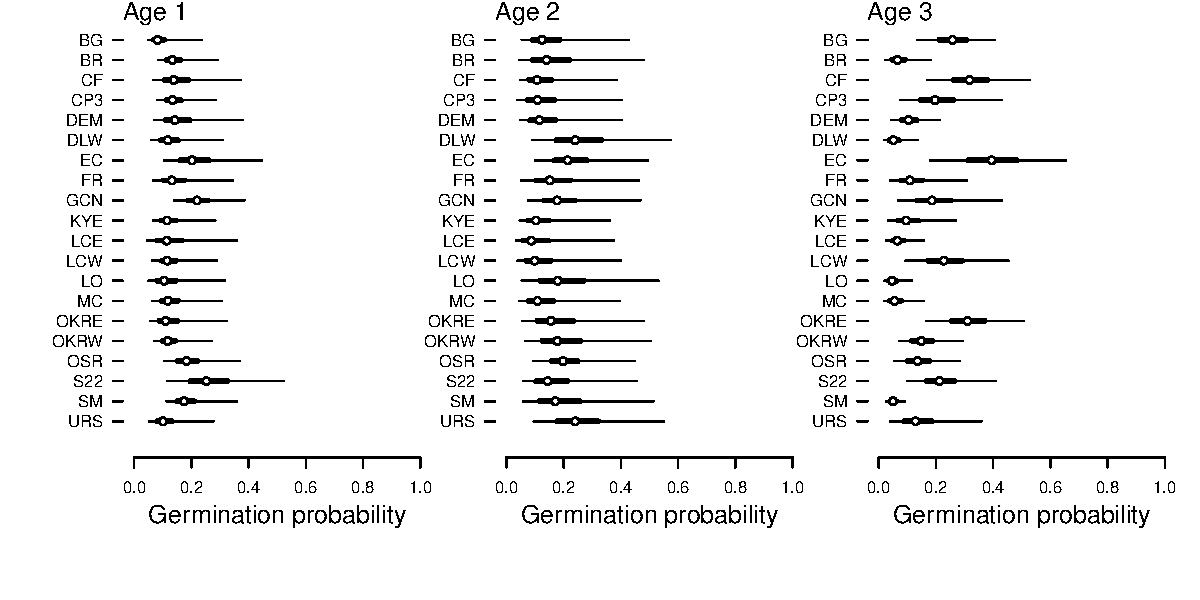
\includegraphics[page=1,width=\textwidth]{../../figures/germination-population.pdf} 
        \includegraphics[page=2,width=\textwidth]{../../figures/germination-population.pdf} 
            \caption{ The population-level probability of germination conditional on persistence. (A: top row) Age-specific germination probabilities for each population. (B: bottom row) Age-specific germination probabilities for each population plotted against the population geographic position. In all graphs, the points are the median of the posterior. Uncertainty about the estimate is summarized by the 50\% (thick line) and 95\% credible intervals (thin lines). }
 \label{fig:germination-estimates-population}
\end{figure}

 \begin{figure}[!h]
        \centering
        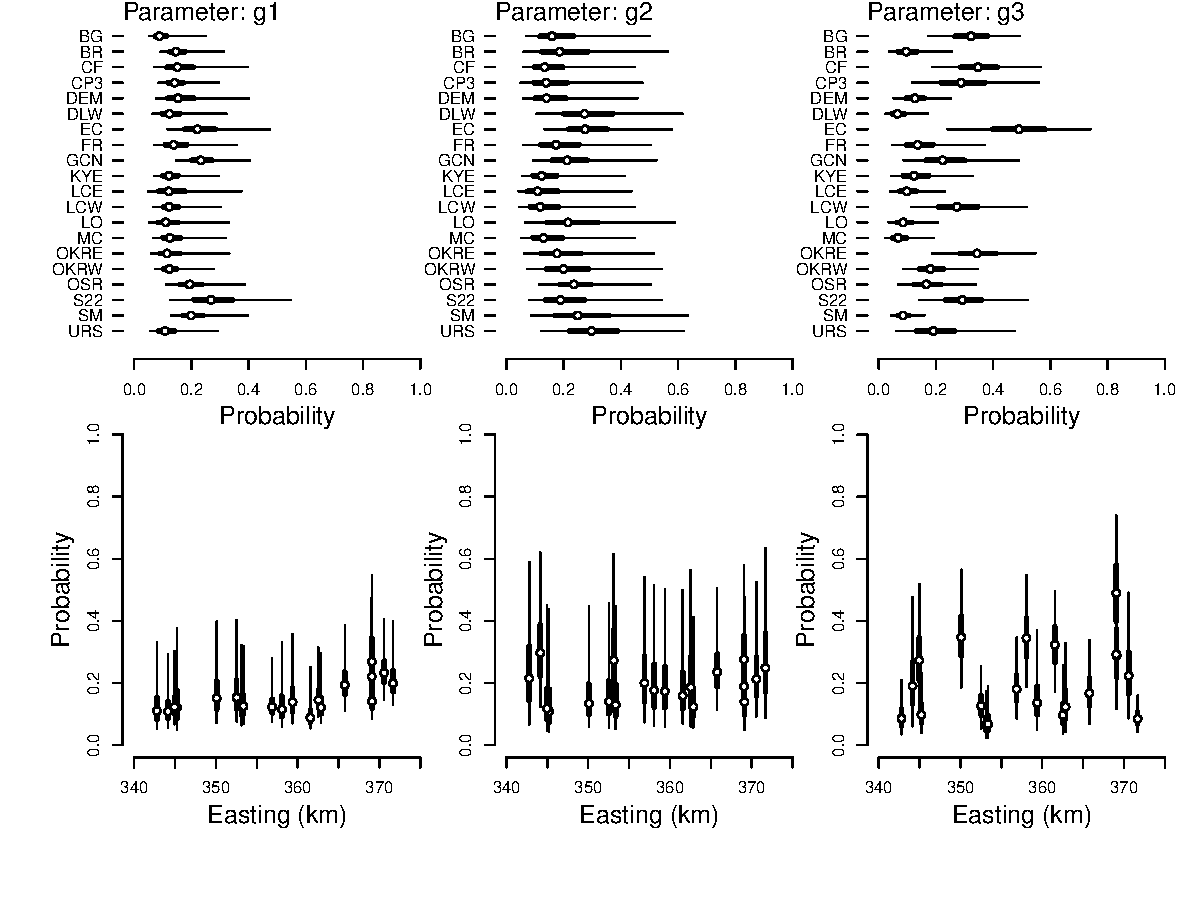
\includegraphics[page=1,width=.9\textwidth]{../../figures/structured-parameters-all.pdf} 
            \caption{ The population-level probability of germination conditional on persistence and viability. (A: top row) Age-specific germination probabilities for each population. (B: bottom row) Age-specific germination probabilities for each population plotted against the population geographic position. In all graphs, the points are the median of the posterior. Uncertainty about the estimate is summarized by the 50\% (thick line) and 95\% credible intervals (thin lines). }
 \label{fig:germination-estimates-population}
\end{figure}

 \begin{figure}[!h]
        \centering
        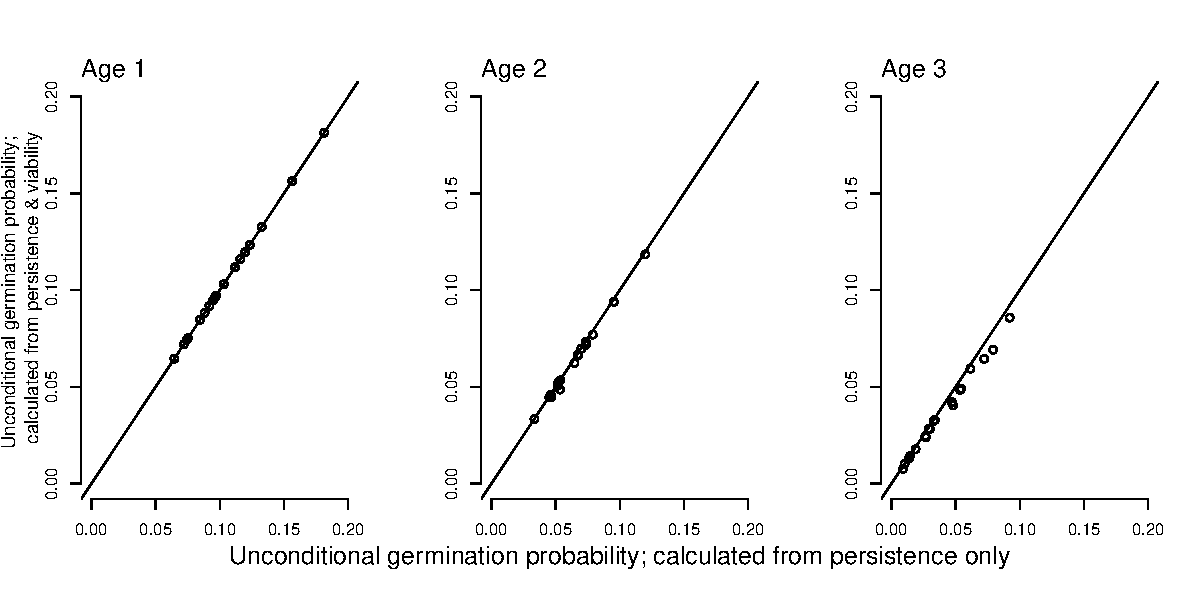
\includegraphics[page=1,width=\textwidth]{../../figures/compare-structured-germination.pdf} 
        \includegraphics[page=2,width=\textwidth]{../../figures/compare-structured-germination.pdf} 
            \caption{ Comparison of conditional and unconditional estimates of germination. (A: top row) Unconditional germination probabilities calculated from estimates conditional on persistence only versus unconditional germination probabilities calculated from estimates conditional on persistence and viability. (B: bottom row) Conditional germination probabilities calculated from estimates conditional on persistence only versus conditional germination probability calculated from estimates conditional on persistence and viability. In all graphs, the points are the median of the posterior. Values on the 1:1 line indicate that estimates are identical; values below the 1:1 line indicate the estimate on the y-axis is greater than the estimate on the x-axis. Values above the 1:1 line indicate the estimate on the y-axis is less than the estimate on the x-axis. }
 \label{fig:germination-estimates-population}
\end{figure}


 \begin{figure}[!h]
        \centering
        \includegraphics[page=2,width=\textwidth]{../../figures/compare-structured-germination2.pdf} 
            \caption{ Conditional germination probabilities calculated from estimates conditional on persistence only (black, open points, dotted lines) compared to conditional germination probabilities calculated from estimates conditional on persistence and viability (orange, solid points, solid lines). In all graphs, the points are the median of the posterior and uncertainty about the estimate is summarized by the 95\% credible intervals.  }
 \label{fig:germination-estimates-population}
\end{figure}

%%%%%%%%%%%%%%%%%%%%%%%%%%%%%%%%%%%%%%%%%%%%%%%%%%%%
% Survival
%%%%%%%%%%%%%%%%%%%%%%%%%%%%%%%%%%%%%%%%%%%%%%%%%%%%

 \begin{figure}[!h]
        \centering
        \includegraphics[page=2,width=\textwidth]{../../figures/structured-parameters-all.pdf} 
            \caption{ The population-level probability of winter survival for seeds of age 1 ($s_1$), age 2 ($s_3$), and age 3 ($s_5$) conditional on persistence and viability. (A: top row) Survival probabilities for each population. (B: bottom row) Survival probabilities for each population plotted against the population geographic position. In all graphs, the points are the median of the posterior. Uncertainty about the estimate is summarized by the 50\% (thick line) and 95\% credible intervals (thin lines). }
 \label{fig:germination-estimates-population}
\end{figure}

 \begin{figure}[!h]
        \centering
        \includegraphics[page=3,width=\textwidth]{../../figures/structured-parameters-all.pdf} 
            \caption{ The population-level probability of summer survival for seeds of age 1 ($s_2$), age 2 ($s_4$), and age 3 ($s_6$) conditional on persistence and viability. (A: top row) Survival probabilities for each population. (B: bottom row) Survival probabilities for each population plotted against the population geographic position. In all graphs, the points are the median of the posterior. Uncertainty about the estimate is summarized by the 50\% (thick line) and 95\% credible intervals (thin lines). }
 \label{fig:germination-estimates-population}
\end{figure}

 \begin{figure}[!h]
        \centering
        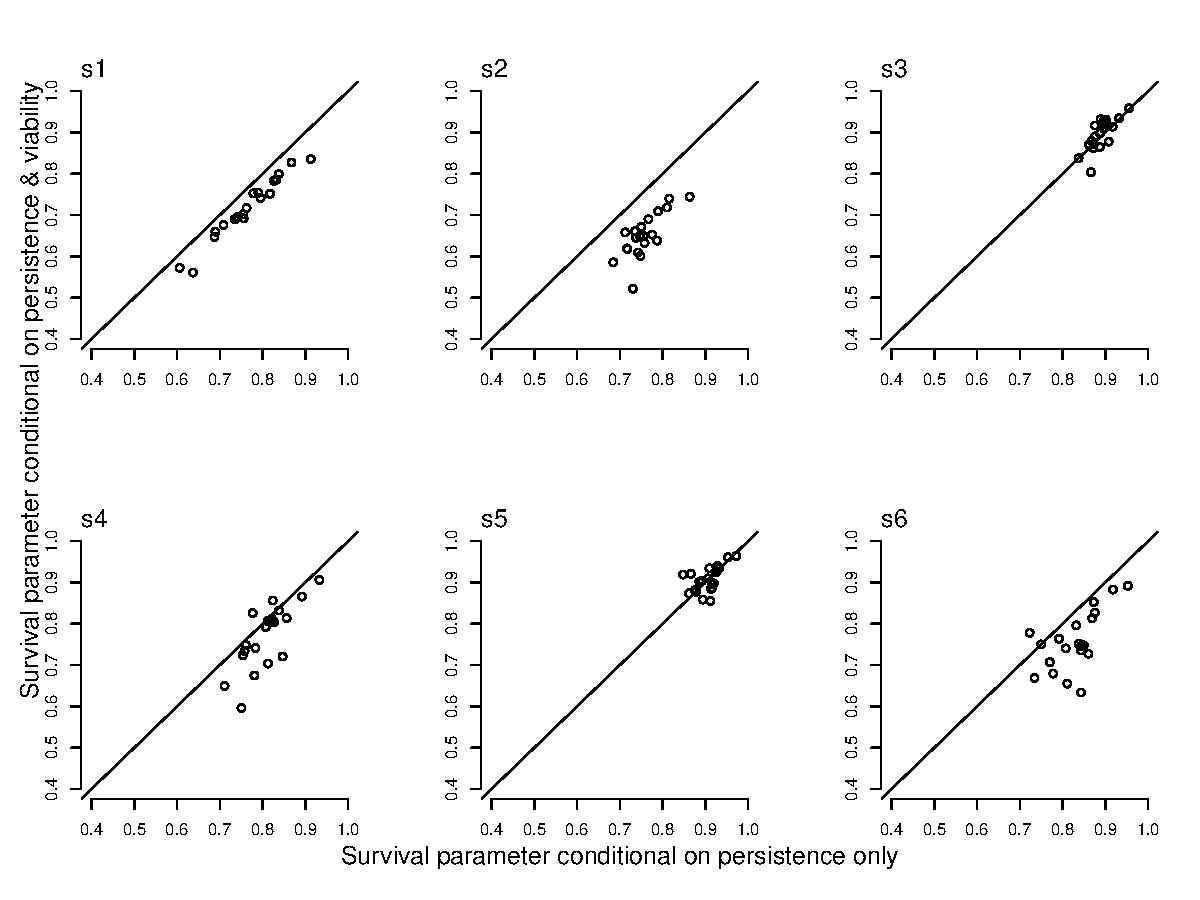
\includegraphics[page=1,width=\textwidth]{../../figures/compare-structured-survival.pdf} 
            \caption{ Survival probabilities calculated from estimates conditional on persistence only compared to survival probabilities calculated from estimates conditional on persistence and viability. In all graphs, the points are the median of the posterior. Values on the 1:1 line indicate that estimates are identical; values below the 1:1 line indicate the estimate on the y-axis is greater than the estimate on the x-axis. Values above the 1:1 line indicate the estimate on the y-axis is less than the estimate on the x-axis. }
 \label{fig:germination-estimates-population}
\end{figure}


 \begin{figure}[!h]
        \centering
        \includegraphics[page=2,width=\textwidth]{../../figures/compare-structured-survival2.pdf} 
            \caption{  Survival probabilities calculated from estimates conditional on persistence only (black, open points, dotted lines) compared to survival probabilities calculated from estimates conditional on persistence and viability (orange, solid points, solid lines). In all graphs, the points are the median of the posterior and uncertainty about the estimate is summarized by the 95\% credible intervals.  }
 \label{fig:germination-estimates-population}
\end{figure}

%%%%%%%%%%%%%%%%%%%%%%%%%%%%%%%%%%%%%%%%%%%%%%%%%%%%
% Some more comparisons
%%%%%%%%%%%%%%%%%%%%%%%%%%%%%%%%%%%%%%%%%%%%%%%%%%%%

 \begin{figure}[!h]
        \centering
        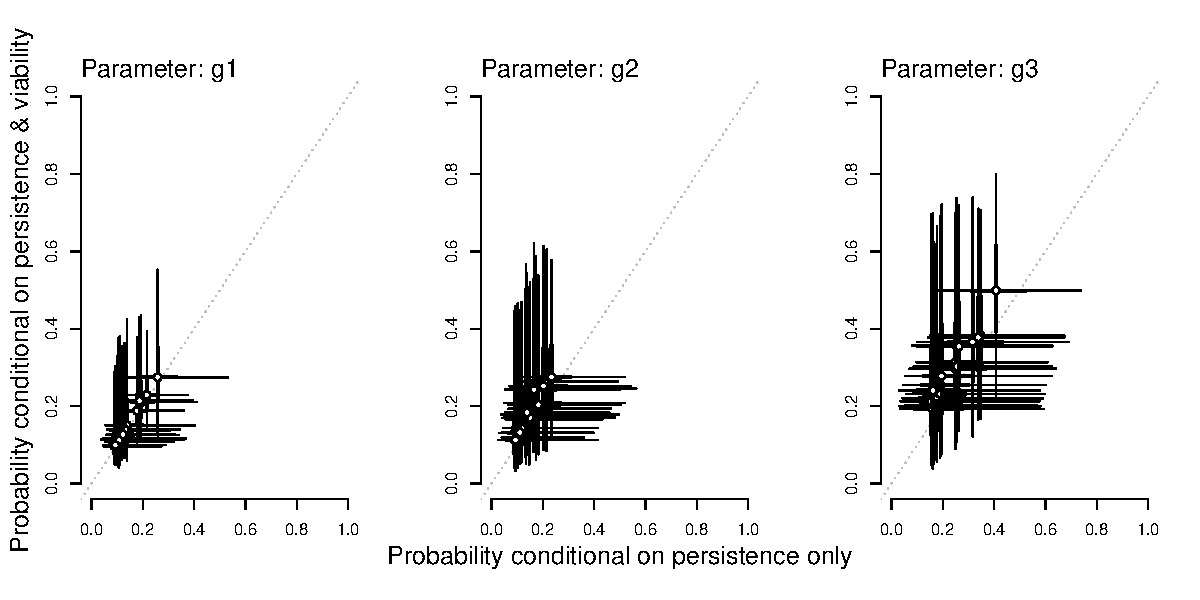
\includegraphics[page=1,scale=.5]{../../figures/compare-structured-parameters-1to1.pdf} 
        \includegraphics[page=2,scale=.5]{../../figures/compare-structured-parameters-1to1.pdf} 
        \includegraphics[page=3,scale=.5]{../../figures/compare-structured-parameters-1to1.pdf} 
            \caption{  Comparison of structured model parameters estimated with and without accounting for viability.  }
 \label{fig:germination-estimates-population}
\end{figure}


%%%%%%%%%%%%%%%%%%%%%%%%%%%%%%%%%%%%%%%%%%%%%%%%%%%%
% Summary
%%%%%%%%%%%%%%%%%%%%%%%%%%%%%%%%%%%%%%%%%%%%%%%%%%%%

 \begin{figure}[!h]
   \centering
       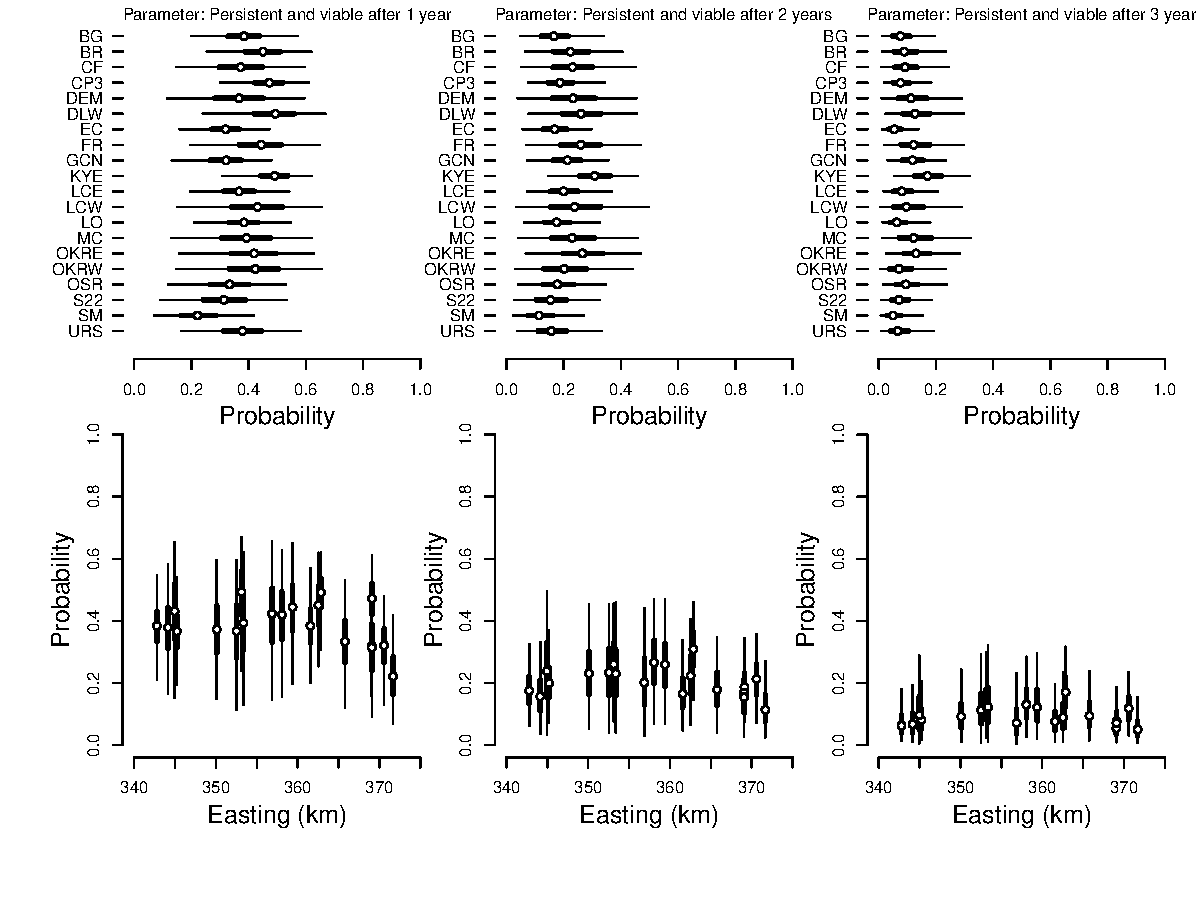
\includegraphics[page=1,width=\textwidth]{../../figures/cumulative-survival.pdf}  
    \caption{ The population-level survival function is used to estimate the probability that seeds in each population persist and are viable after 1, 2, or 3 years in the soil. In all graphs, the points are the median of the posterior. Uncertainty about the estimate is summarized by the 50\% (thick line) and 95\% credible intervals (thin lines). }
 \label{fig:viability-estimates-population}
\end{figure}

 \begin{figure}[!h]
   \centering
       \includegraphics[page=2,width=\textwidth]{../../figures/cumulative-survival.pdf}  
    \caption{ The population-level survival function is used to estimate the probability that seeds in each population persist after 1, 2, or 3 years in the soil. In all graphs, the points are the median of the posterior. Uncertainty about the estimate is summarized by the 50\% (thick line) and 95\% credible intervals (thin lines). }
 \label{fig:viability-estimates-population}
\end{figure}

\clearpage
\newpage

%%%%%%%%%%%%%%%%%%%%%%%%%%%%%%%%%%%%%%%%%%%%%%%%%%%%
% Aboveground
%%%%%%%%%%%%%%%%%%%%%%%%%%%%%%%%%%%%%%%%%%%%%%%%%%%%
\subsection*{Aboveground}


 \begin{figure}[!h]
   \centering
       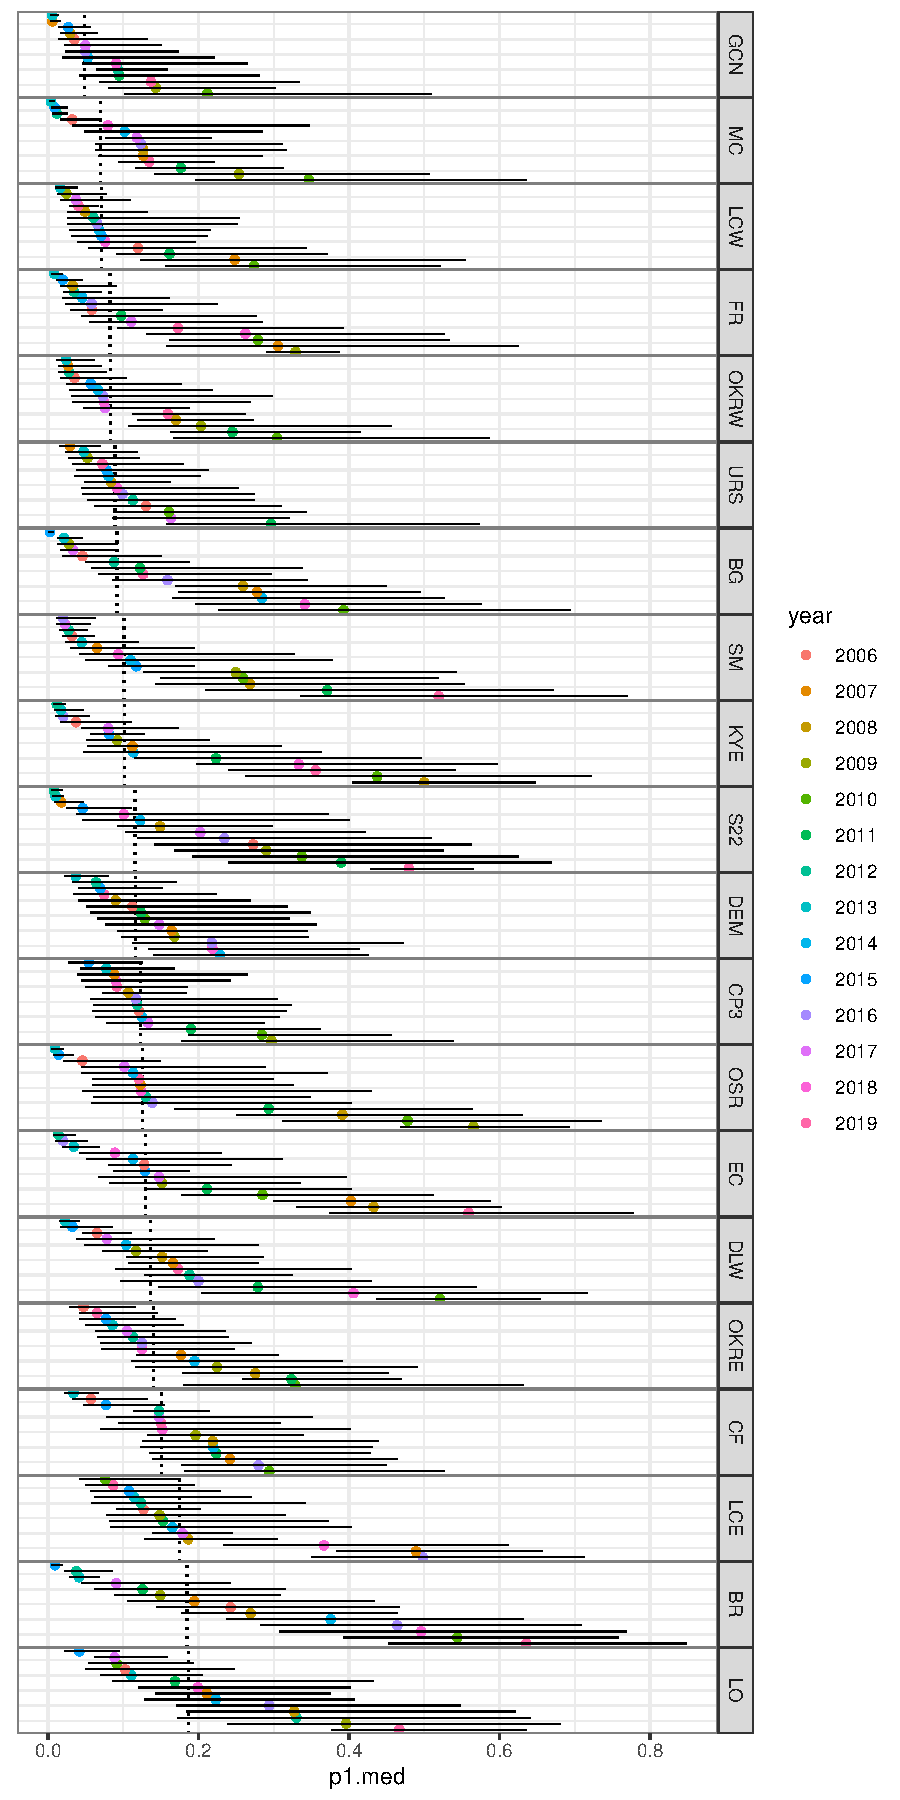
\includegraphics[page=1,height=.95\textheight]{../../figures/interannual-sigma.pdf}  
    \caption{ Interannual estimates of median seedling survival to fruiting. Credible intervals are the 95\% highest posterior density intervals. }
 \label{fig:viability-estimates-population}
\end{figure}

 \begin{figure}[!h]
   \centering
       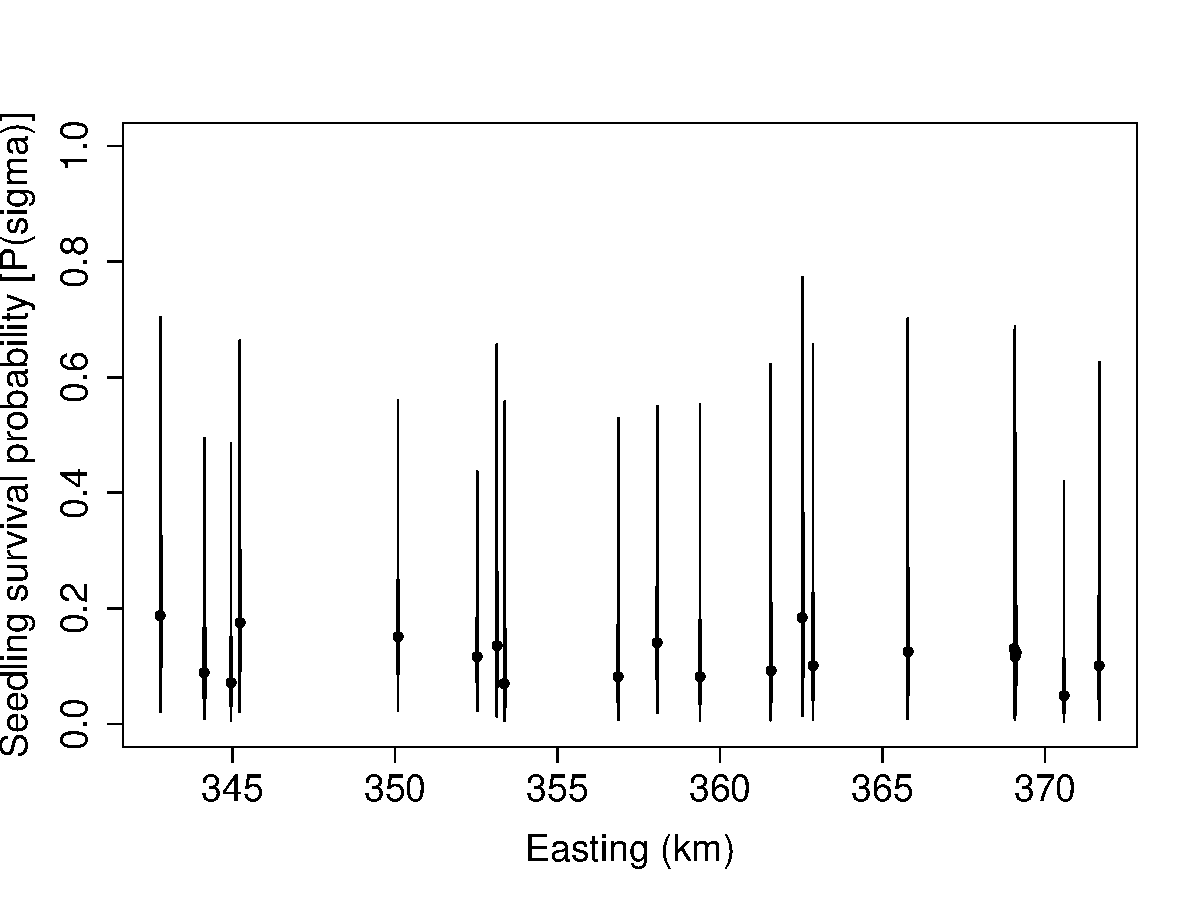
\includegraphics[page=1,width=\textwidth]{../../figures/spatial-sigma.pdf}  
    \caption{ Population-level estimates of median seedling survival to fruiting. Credible intervals are the 95\% highest posterior density intervals. }
 \label{fig:viability-estimates-population}
\end{figure}

 \begin{figure}[!h]
   \centering
       \includegraphics[page=1,height=.95\textheight]{../../figures/interannualTFEfull.pdf}  
    \caption{ Interannual estimates of total fruit equivalents per plant (TFE). From 2006-2012, TFE was estimated in the field; from 2013-2018, TFE was calculated from counts of damaged and undamaged fruits per plant. Credible intervals are the 95\% highest posterior density intervals. }
 \label{fig:viability-estimates-population}
\end{figure}

 \begin{figure}[!h]
   \centering
       \includegraphics[page=1,width=\textwidth]{../../figures/spatialTFEfull.pdf}  
    \caption{ Interannual estimates of total fruit equivalents per plant (TFE). From 2006-2012, TFE was estimated in the field; from 2013-2018, TFE was calculated from counts of damaged and undamaged fruits per plant. Credible intervals are the 95\% highest posterior density intervals. }
 \label{fig:viability-estimates-population}
\end{figure}

 \begin{figure}[!h]
   \centering
       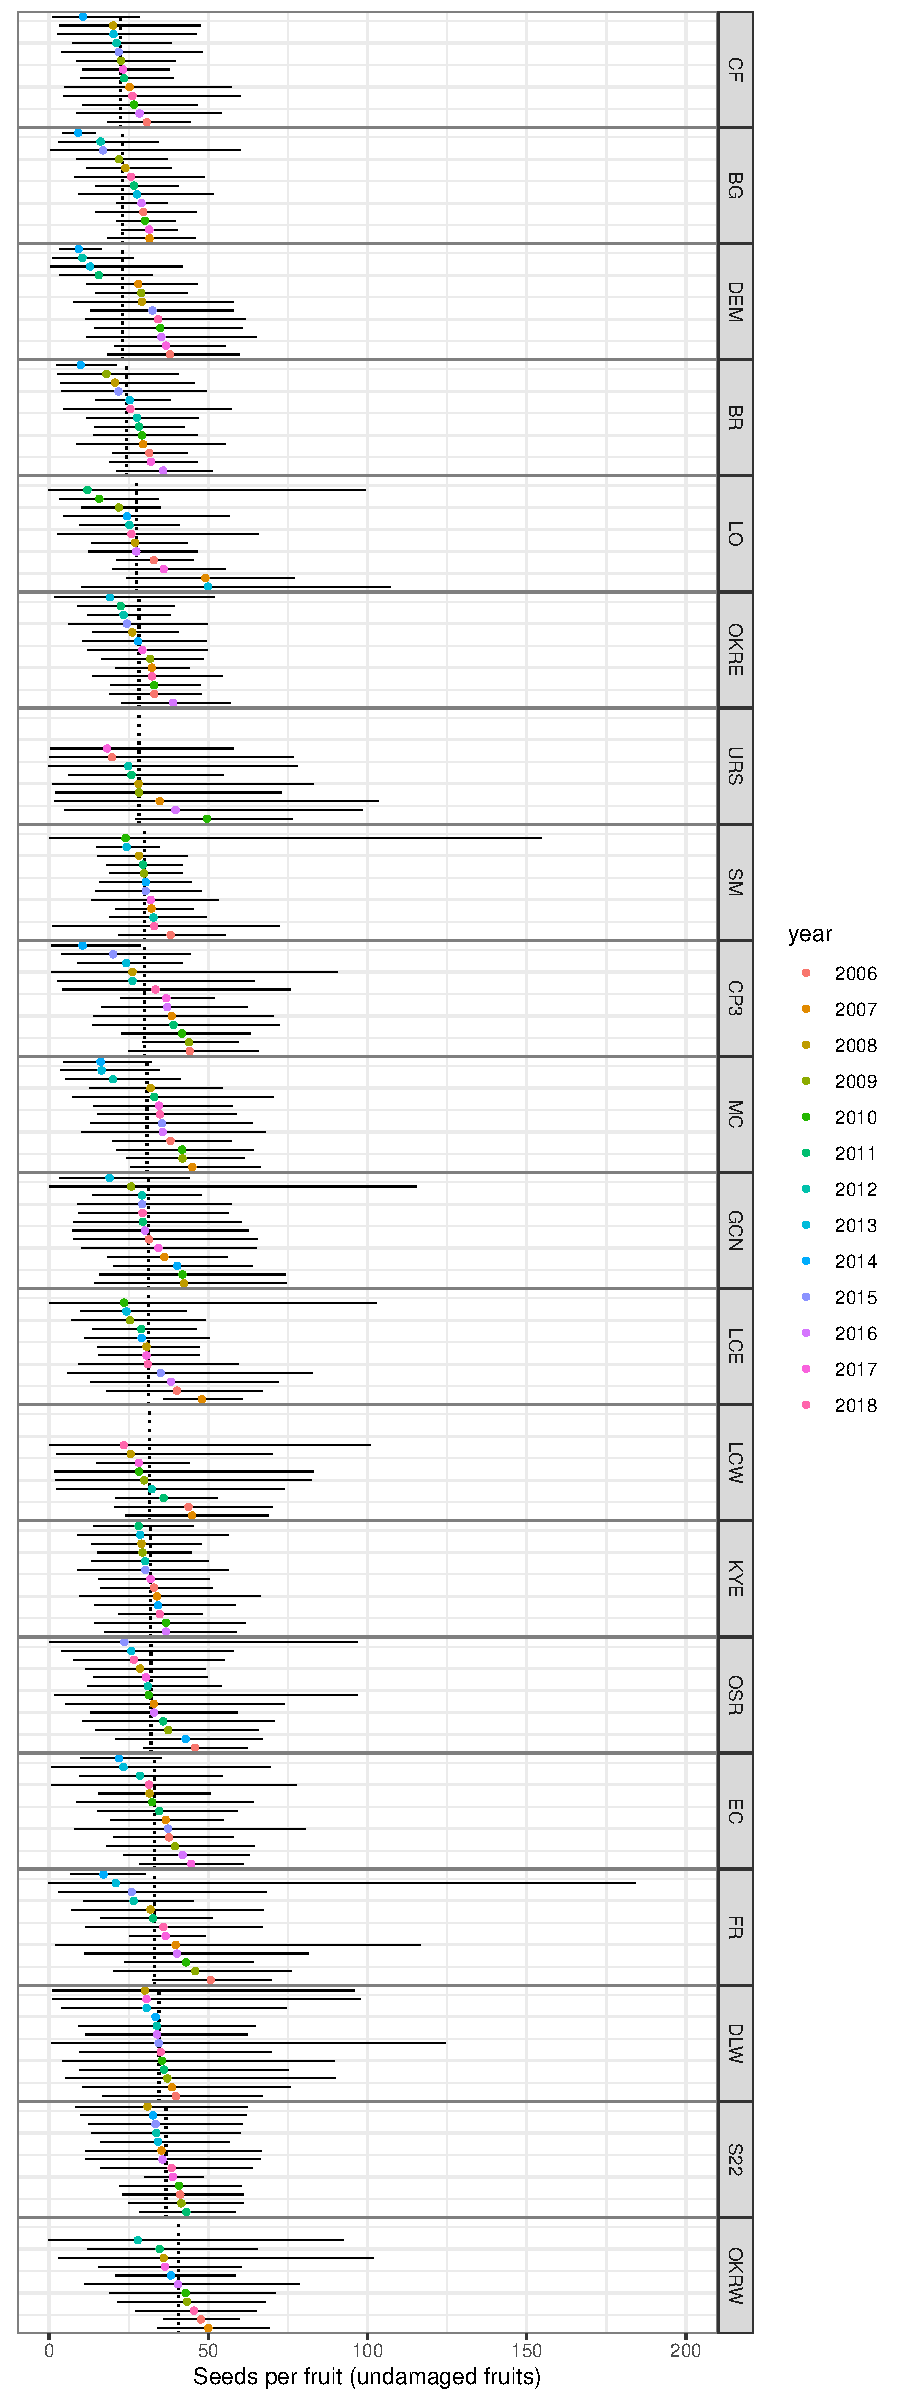
\includegraphics[page=1,height=.95\textheight]{../../figures/interannualSeeds.pdf}  
    \caption{ Interannual estimates of median seeds per undamaged fruit. Credible intervals are the 95\% highest posterior density intervals. }
\end{figure}

 \begin{figure}[!h]
   \centering
       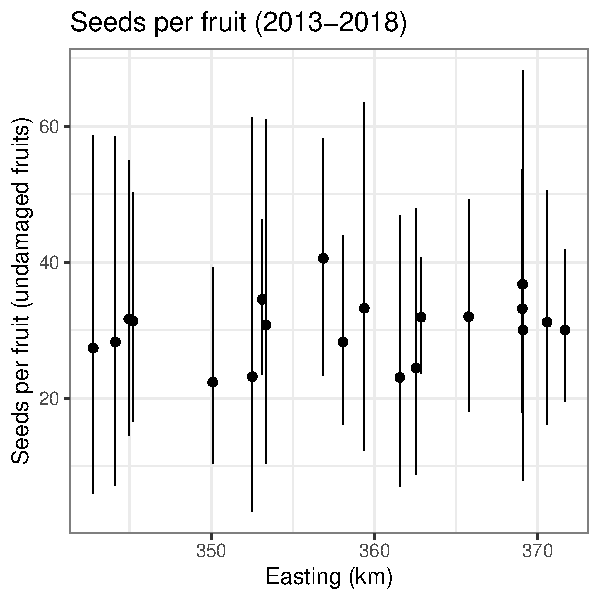
\includegraphics[page=1,width=\textwidth]{../../figures/spatialSeeds.pdf}  
    \caption{ Population-level estimates of median seeds per undamaged fruit. Credible intervals are the 95\% highest posterior density intervals. }
\end{figure}

\clearpage
\newpage
%%%%%%%%%%%%%%%%%%%%%%%%%%%%%%%%%%%%%%%%%%%%%%%%%%%%
% Analysis
%%%%%%%%%%%%%%%%%%%%%%%%%%%%%%%%%%%%%%%%%%%%%%%%%%%%
\subsection*{Analysis}

 \begin{figure}[!h]
   \centering
%       \includegraphics[page=2,width=\textwidth]{f}  
    \caption{ Correlation of germination and seed survival. }
 \label{fig:viability-estimates-population}
\end{figure}

 \begin{figure}[!h]
   \centering
%       \includegraphics[page=2,width=\textwidth]{f}  
    \caption{ Correlation of germination and variance in reproductive success. }
 \label{fig:viability-estimates-population}
\end{figure}

 \begin{figure}[!h]
   \centering
%       \includegraphics[page=2,width=\textwidth]{f}  
    \caption{ Expected germination from DI model vs. observed germination from DI model. }
 \label{fig:viability-estimates-population}
\end{figure}

\end{document}